\documentclass[12pt,letterpaper,final,titlepage]{article}
%\documentclass[12pt,letterpaper,draft]{article}
\usepackage[utf8]{inputenc}
\usepackage[spanish]{babel}
\author{Las mil secciones son para no perderme durante la escritura}
\title{}
%\date{\today}
\date{}
%>>> Mate, símbolos
\usepackage{amsmath}
\usepackage{amssymb}
\usepackage{amsfonts}
\usepackage{mathtools}
\usepackage{newtxmath} % fuente?
\usepackage{array}
\usepackage{multirow} % tablas
\usepackage{tabularx} % tablas
%<<< Mate, símbolos
%>>> Bibliografía
\usepackage{csquotes} % citar
%\usepackage[backend=biber,style=alphabetic,sorting=nyt]{biblatex} % OVERLEAF
%\addbibresource{bibfile.bib} % OVERLEAF
\usepackage[backend=bibtex,style=alphabetic]{biblatex} % genérico no-overleaf
\usepackage{apacite}
%\bibliographystyle{apacite}
\bibliography{pro} % genérico no-overleaf
%>>>  Bibliografía
%>>> Imágenes
\usepackage{graphicx} % insertar
\usepackage{float} % ubicación flotante
%>>> Imágenes
%>>> Clickable hypers
\usepackage{hyperref}
\hypersetup{
    hyperindex=true,
    linktocpage=false,
    colorlinks=true,
    allcolors=black,
    bookmarksnumbered=true,
    unicode=true,
}
%<<< Clickable hypers
%>>> notas verticales QUITAR AL FINAL
%\usepackage{marginnote}
\usepackage{geometry}
\geometry{marginparwidth=.45cm,marginparsep=.45cm} %NO TOCAR EL PRIMER .45, constante
\newcommand{\notad}[1]{\normalmarginpar\marginpar{\rotatebox{90}{$\uparrow$ #1}}}
%
\newcommand{\notai}[1]{\reversemarginpar\marginpar{\rotatebox{90}{$\downarrow$ #1}}}
%
\newcommand{\notadhi}[1]{\normalmarginpar\marginpar{\rotatebox{270}{$\downarrow$ #1}}}
%
\newcommand{\notaihi}[1]{\reversemarginpar\marginpar{\rotatebox{270}{$\uparrow$ #1}}}
%<<< notas verticales QUITAR AL FINAL
%CIRCULOS
\usepackage{tikz}
\usetikzlibrary{shapes}
%%\usepackage[export]{adjustbox}
\usepackage{subcaption}
\usepackage{wasysym}
\usepackage{multicol}
%
%\usepackage[table]{xcolor}
\usepackage{microtype} %font kerning, poner atención
\usepackage{wrapfig}
\title{Modelo para procesamiento de lenguage natural*\citadhi{?}}
\begin{document}
\maketitle
\renewcommand{\abstractname}{Resumen ejecutivo}\begin{abstract}
El uso de las redes sociales en el mundo ha generado la aparición de estudios enfocados a un sinnúmero de casos y aplicaciones. Estos estudios van siempre acompañados por técnicas de Procesamiento de Lenguaje Natural, unos más sofisticados y otros más básicos, a partir de palabras simples, considerando cierto tipo de personajes, considerando el uso de temas “hashtag”, en diferentes rangos de fechas, con enfoque de sentimientos, entre muchos otros casos. Pero de que sirve el Procesamiento de Lenguaje Natural sin un modelo estadístico que describa numéricamente lo que está sucediendo con las muestras de textos, como porque se dice algo repetidamente, o que hay en común en la opinión de la gente o de los reporteros, o cuál es la tendencia social y así sucesivamente. La estadística en esta propuesta de modelo tiene dos intervenciones. La primera es al inicio del proceso, con una estimación de lo que se pretende obtener y la segunda es con una comprobación de dicha estimación y en su caso una retroalimentación para asegurar ciertos valores usando aprendizaje de máquina y ajustando parámetros de categorización y diversificación de palabras, buscando confirmar o rechazar una suposición, con elementos numéricos bien fundamentados.
\end{abstract}

%\tableofcontents
\section {Marco teórico}\label{sec:marco}
\subsection {Modelo relacional de base de datos}\label{subsec:rdb}
El \emph{modelo relacional de base de datos}, consiste en cinco componentes:
\begin{enumerate}
	\item Una colección de tipos escalares, pueden ser definidos por el sistema (INTEGER, CHAR, BOOLEAN, etc.) o por el usuario.
	\item Un generador de tipos de relaciones y un intérprete para las relaciones mismas.
	\item Estructuras para definir variables relacionales de los tipos generados.
	\item Un operador para asignar valores de relación a dichas variables.
	\item Una colección relacionalmente completa para obtener valores relacionales de otros valores relacionales mediante operadores relacionales genéricos.
\end{enumerate}
Aunque tersa esta lista es útil para delimitar lo que el modelo relacional es y no es.\\
Se debe comenzar definiendo los \emph{tipos}, ya que las relaciones se definen sobre ellos, son ``en esencia un conjunto finito de valores nombrados\textemdash todos los valores posibles de alguna categoría específica(...)''\cite{date12}.

Los \emph{atributos} son pares ordenados de combinaciones atributo-nombre/tipo-nombre y una \emph{tupla} es un par ordenado de atributos.
El modelo relacional también soporta varios tipos de \emph{llaves}, que poseen las propiedades de unicidad, ninguna contiene dos tuplas distintas con el mismo valor e irreductibilidad, ningún subconjunto suyo es tiene unicidad.
%La llave foránea (\emph{FK}) es una combinación o set se atributos FK en una relación $r2$ tal que se requiere que cada valor FK sea igual a algún valor de alguna llave K en alguna relación $r1$ ($r1$ y $r2$ no son necesariamente distintos).
\begin{table}[H]\centering\begin{tabular}{rc|c|c|l}
		\cline{2-4}
		\multicolumn{1}{r}{$\text{Atributos}\begin{cases}\ \end{cases}$}&\multicolumn{1}{|c|}{código}&\multicolumn{1}{c|}{fecha}&\multicolumn{1}{c|}{estado}&\multicolumn{1}{l}{}\\
		\cline{2-4}
		\multirow{3}{*}{$\text{Tuplas}\begin{cases}\\\\\end{cases}$}&\multicolumn{1}{|c|}{MX01}& 29-07-99&1&\multicolumn{1}{ l }{}\\
		\cline{2-4}
		&\multicolumn{1}{|c|}{MX02}&30-07-99&1&\multicolumn{1}{ l }{}\\
		\cline{2-4}
		&\multicolumn{1}{|c|}{MX03}&31-07-99&0&\multicolumn{1}{ l }{}\\
		\cline{2-4}
	\end{tabular}\caption{Representación de una tabla de una base en datos, la fila superior muestra tres atributos distintos y \emph{cada una} de las filas siguientes es una tupla.}\label{table:tupla}\end{table}
La \emph{restricción de integridad} (\emph{constraint}) es una expresión booleana que debe evaluarse como verdadera. Los \emph{constraints de tipo} definen los valores que constituyen un tipo dado y los \emph{constraints de base de datos} limitan los valores que pueden aparecer en cierta base de datos. Las bases de datos suelen tener múltiples constraints específicos, expresados en términos de sus relaciones, sin embargo, el modelo relacional incluye dos constraints genéricos, que aplican a cada base de datos:
\begin{itemize}
	\item Regla de integridad de identidad: Las \emph{llaves primarias} (\emph{PK}) deben ser no nulas.
	\item Regla de integridad de referencia: Las \emph{llaves foráneas} (\emph{FK}) deben tener relación (si $B$ referencia a $A$, $A$ debe existir).
\end{itemize}

Las operaciones del modelo relacional están cimientadas en el \emph{álgebra relacional}, las operaciones primitivas del álgebra producen nuevas relaciones, que pueden manipularse también por medio de operaciones del álgebra mismo. Una secuencia de operaciones de álgebra relacional forma una \emph{expresión de álgebra relacional} cuyo resultado es una relación que representa el resultado de una consulta (o solicitud de consulta) de base de datos.\cite{elma11} Estas operaciones pueden clasificar en dos grupos, operaciones de conjuntos*\notadhi{(así se llaman? checar libro en l'espagnol)``set operations''} de la teoría de conjuntos matemáticos refiere a la operaciones \emph{UNION}, \emph{INTERSECTION}, \emph{SET DIFFERENCE} (\emph{MINUS}) y \emph{CARTESIAN PRODUCT} (\emph{CROSS PRODUCT}). El otro grupo consiste en operaciones específicas para bases de datos relacionales: \emph{JOIN}, \emph{SELECT} y \emph{PROJECT}. Estas dos últimas, por operar con una sola relación, son también conocidas como \emph{operaciones unarias}.

SELECT elige un subconjunto de tuplas de una relación que satisfacen la condición de selección
\begin{equation}
\sigma_\text{\textless condición de selección\textgreater}{\text{(R)}}
\end{equation}
donde $\sigma$ denota el operador SELECT, y la condición de selección es una expresión booleana especificada en los atributos de la relación $R$.

PROJECT produce una nueva relación de atributos y tuplas*\notaihi{se explican hasta modelo rel, en los libros se explica primero} duplicadas
\begin{equation}
\pi_\text{\textless lista de atributos\textgreater}{\text{(R)}}
\end{equation}
donde $\pi$ es el denota el operador PROJECT y la lista de atributos es la sublista de atributos deseados de la relación $R$.

Las operaciones con dos relaciones reciben el nombre de \emph{operaciones binarias}. Si las relaciones $R(A_1,A_2,\ldots,A_n)$ y $S(B_1,B_2,\ldots,B_n)$ son compatibles de unión (tienen el mismo grado $n$ y $dom(A_i)=dom(B_i)$ para $1\leq i\leq n$) podemos usarlas para definir las siguientes operaciones binarias:
\begin{itemize}
	\item UNION: El resultado de esta operación se denota $R \cup S$, es una relación que incluye todas las tuplas que están en $R$, $S$ o ambos, se eliminan duplicados.
	\item INTERSECTION: El resultado de esta operación se denota $R \cap S$, es una relación que incluye todas las tuplas que están en ambos $R$ y $S$.
	\item SET DIFFERENCE: El resultado de esta operación se denota $R - S$, es una relación que incluye todas las tuplas que están en ambos $R$ pero no en $S$.
\end{itemize}

El operador CARTESIAN PRODUCT, denotado $R \times S$ es la operación binaria que no requiere compatibilidad de unión y produce un nuevo elemento al combinar cada miembro (tupla) de cada relación conjunto) con cada otro miembro de la otra relación. El resultado de $R(A_1,A_2,\ldots,A_n)$ y $S(B_1,B_2,\ldots,B_m)$ es una relación $Q$ con atributos $Q(A_1,A_2,\ldots,A_n,B_1,B_2,\ldots,B_m)$ (en ese orden) de grado $n+m$. El resultado $Q$ tiene una tupla por cada combinación de tuplas de $R$ y $S$.

JOIN $\Join$, es el operador utilizado para combinar tuplas relacionadas de dos relaciones en una sola tupla. Pertinente para procesar relaciones entre relaciones. Si tenemos dos relaciones $R(A_1,A_2,\ldots,A_n)$ y $S(B_1,B_2,\ldots,B_m)$ podemos escribir la operación JOIN como
\begin{equation}
R\Join_\text{\textless condiciones de unión\textgreater}S
\end{equation}
el resultado de la unión es la relación $Q$ con atributos $Q(A_1,A_2,\ldots,A_n,B_1,B_2,\ldots,B_m)$ (en ese orden). El resultado $Q$ tiene una tupla por cada combinación de tuplas de $R$ y $S$ que satisfacen las condiciones de unión.
\begin{wrapfigure}{r}{4.4cm}
	\begin{tikzpicture}
	\def\IA{(0,0) circle (2.2cm)}
	\def\AM{(270:1.0cm) circle (1.2cm)}
	\def\AP{(270:1.52cm) circle (.675cm)}
	\draw \IA node[above]{\small $\overset{\text{Inteligencia artificial}}{}$};
	\draw \AM node[above]{\scriptsize $\overunderset{\text{Aprendizaje}}{\text{maquinal}}{}$};
	\draw \AP node{\tiny $\overunderset{\text{Aprendizaje}}{\text{profundo}}{}$};
	\end{tikzpicture}\caption[Inteligencia Artificial]{AP$\subset$AM$\subset$IA}
\end{wrapfigure}\label{fig:AI}\subsection {AI, ML, NLP}\label{subsec:intela}
\emph{Inteligencia artificial (IA)} es ``el esfuerzo por automatizar tareas intelectuales normalmente realizadas por humanos''\cite{cho18}, de este campo general se desprenden el \emph{aprendizaje maquinal (AM)} y \emph{aprendizaje profundo (AP)}.
%\begin{figure}[H]\centering
%\begin{tikzpicture}
%\def\IA{(0,0) circle (1.5cm)}
%\def\AM{(270:.7cm) circle (.75cm)}
%\def\AP{(270:1.025cm) circle (.375cm)}
%\draw \IA node[above]{IA};
%\draw \AM node[above]{AM};
%\draw \AP node{AP};
%\end{tikzpicture}
%\caption{Aprendizaje profundo (AP), es un subcampo del aprendizaje maquinal (AM), que a su vez es un subcampo de la inteligencia artificial (IA)\cite{cho18}.}\label{fig:AI}
%\end{figure}

Tom Mitchell \cite{mich19} define aprendizaje maquinal como ``un programa de computadora aprende de experiencia $E$ con respecto a una tarea $T$ y una medición de rendimiento $P$, si su rendimiento en $T$, medido por $P$, mejora con $E$.''

A diferencia del paradigma clásico de programación donde los humanos introducen datos y órdenes para procesarlos, un sistema de aprendizaje maquinal no se programada explícitamente, se introducen muchos ejemplos relevantes a una tarea (datos y respuestas esperadas) con los que es entrenado y si encuentra una estructura estadística en ellos, genera una regla para automatizar la tarea.

El \emph{procesamiento de lenguaje natural (PLN)}, es el conjunto de métodos para hacer accesible el lenguaje humano a las computadoras\cite{eise19}. Toma conocimientos de muchas tradiciones intelectuales, como lingüística y teoría formal del lenguaje, autómatas y otras áreas computación, inteligencia artificial, aprendizaje maquinal y profundo, estadística, teoría de la información, fonética y fonología, estas dos últimas áreas son de particular utilidad para procesamiento de voz. Existen dos posturas opuestas sobre lo que la tarea principal del PLN debe ser:
\begin{itemize}
	\item Entrenar sistemas de principio a fin para que transmuten texto sin procesar en cualquier estructura deseada.
	\item Transformar texto en una pila de estructuras lingüísticas de uso general que en teoría deben poder soportar cualquier aplicación.
\end{itemize}
En la actualidad no hay consenso y ambos tipos de sistemas se consideran viables, este proyecto se basará en el segundo paradigma. 

Por lo general el PLN divide sus funciones en módulos para facilitar la reutilización de algoritmos genéricos en diversas tareas y modelos, dos de los módulos básicos son \emph{búsqueda} y \emph{aprendizaje} con los que se puede resolver muchos problemas que tienen la forma matemática
\begin{equation}
\begin{matrix}
\hat{y}=argmax\Psi(x,y;0),\\
y\in Y(x)
\end{matrix}\label{EQ:NLP1}
\end{equation}
donde,
\begin{itemize}
	\item $x$ es la entrada, un elemento de un conjunto $X$.
	\item $y$ es el resultado, un elemento de un conjunto $Y$.
	\item $\Psi$ es una función de puntuación (también conocida como \emph{modelo}), que va desde el conjunto $X\times Y$ hasta los números reales.
	\item $\emptyset$ es el vector de parámetros para $\Psi$.
	\item $\hat{y}$ es el resultado previsto, que es elegido para maximizar la función de puntuación.
\end{itemize}
El módulo de búsqueda se encarga de computar el $argmax$ de la función $\Psi$, es decir, encuentra el resultado $\hat{y}$ con la mejor puntuación con respecto a la entrada $x$. El módulo de aprendizaje encuentra los parámetros $\theta$ por medio del procesamiento de grandes conjuntos de datos de ejemplos etiquetados ${\{(x^i,y^i)\}}_{i=1}^{N}$.

Un método lineal de clasificación de texto común es la \emph{bolsa de palabras}, comienza por asignar etiquetas $y\in Y$ donde $Y$ son todas las posibles etiquetas. Se utilizan vectores columna y la fórmula \ref{EQ:NLP1} y puede modelarse con diversas distribuciones (figura \ref{FIG:DISTS}).

Para muchas tareas, las características léxicas (palabras) pierden sentido en aislamiento, por lo que históricamente el PLN se ha enfocado en la clasificación lineal, recientemente algunas tareas pueden resolverse con clasificadores no lineales, es decir, por medio de redes neuronales (aprendizaje profundo).
\subsection {Mate}
Una \emph{variable aleatoria} (v.a.) es una función real $X: \Omega\mapsto\mathbb{R}$ tal que el conjunto $\{\omega\in\Omega:X(\omega)\in I\}$ es un evento de $\Omega$ para cada $I\subset\mathbb{R}$, en un espacio $\Omega$ hipotético. Se le considera \emph{variable aleatoria discreta} (v.a.d.) cuando su rango de valores $R_x$ es finito o contablemente infinito, mientras que una \emph{variable aleatoria continua} (v.a.c.) puede tomar cualquier valor real en un intervalo.

%Una \emph{variable aleatoria} es una función asignando un número real $\mathbb{R}$ a cada posible resultado de un experimento. Con una muestra en espacio $S$, una variable aleatoria $X$ asigna el valor numérico $X(s)$ a cada resultado posible $s$ del experimento. La aleatoriedad viene del hecho que tenemos un experimento aleatorio (con probabilidades descritas por la función de probabilidad $P$). Las variables aleatorias simplifican la notación y expanden la habilidad de cuantificar y resumir resultados de experimentos.

%Se dice que una variable $X$ es discreta cuando si hay una lista finita de valores $a_,a_2,\ldots,a_n$ o un una lista infinita de valores $a_,a_2,\ldots$ de tal forma que $P(X=a_j$ para algún $j)=1$. Si $X$ es una variable aleatoria discreta, entonces el conjunto infinito o contable de valores $x$ tal que $P(X=x)$ se llama \emph{soporte} de $X$. En contraste una variable aleatoria continua puede tomar cualquier valor real en un intervalo.

%\subsubsection{Variable aleatoria comtinua)}
%A diferencia de las variables discretas, las \emph{variables aleatorias continuas} pueden tomar cualquier valor real en un intervalo y tienen una \emph{distribución continua}. Para obtener la probabilidad deseadaWHOMST, se debe integrar la función de densidad de probabilidad sobre el rango apropiado
%\begin{equation}
%P(X\in A)=\int_{A}f(x)dx
%\end{equation}
La forma más natural de expresar la distribución de v.a.d.s es la \emph{función de probabilidad}\cite{blitz19}. Una v.a.d. $X$ con $R_x=\{x_1,x_2x_3,\ldots,x_n,\ldots\}$ tiene una función de distribución
\begin{equation}
\begin{matrix}
f(x)=0\text{ para cada }x \notin R_x\text{;}\\
f(x)=P(X=x)\text{ para } x\in R_x
\end{matrix}\label{eq:FP}
\end{equation}
para una v.a.c. $X$ será una función no negativa real $f:\mathbb{R}\mapsto[0,\infty)$, es decir
\begin{equation}
P(X\in A)=\int_{A}f(x)dx
\end{equation}
%El teorema de \emph{funciones de probabilidad válidas} dice que cuando $X$ es una variable aleatoria con soporte $x1,x2,\ldots$, la función de probabilidad $p_X$ de $x$ debe satisfacer los siguiente criterios:
%\begin{itemize}
%	\item No negativo $p_X (x) > 0$ si $x=x_j$ para un $j$, y $p_X(x)=0$, de otra forma;
%	\item Suma 1: $\sum_{j=1}^{\infty}p_X(x_j)=1$.
%\end{itemize}
%el primer criterio es verdadero porque la probabilidad es no negativa, el segundo es verdadero ya que $X$ debe tomar \emph{algún} valor, y los eventos ${X=xj}$ están disjuntos, entonces
%\begin{equation}
%\sum_{j=1}^{\infty}P(X=x_j)=P\bigg(\bigcup_{j=1}^{\infty}\{X=x_j\}\bigg)=P(X=x_1\ \text{ó}\ X=x_2\ \text{ó}\ \ldots)=1.
%\end{equation}
%Mientras que las distribuciones anteriores nos han dado toda la información acerca de la probabilidad de las variables aleatorias, cuando sólo se requiere un número que extraiga su valor, podemos utilizar la \emph{media}, también conocida como \emph{valor esperado}. Dada una lista de números $x_1,x_2.\ldots,x_n$, para obtener la \emph{media aritmética}, estos se suman y dividen entre $n$:
%\begin{equation}
%\bar{x}=\frac{1}{n}\sum_{j=1}^{n}x_j,
%\end{equation}
%la \emph{media ponderada} de $x_1,x_2.\ldots,x_n$ se obtiene de la siguiente forma:
%\begin{equation}
%\text{media ponderada}(x)=\frac{1}{n}\sum_{j=1}^{n}x_jP_j,
%\end{equation}
%donde los pesos $p_1,p_2.\ldots,p_n$ son números no negativos previamente especificados que suman a $1$.
%\subsubsection {Función de distribución acumulada}
%Esta función describe la distribución de todas las variables aleatorias (a diferencia de la función de probabilidad que sólo se aplica a las discretas). La \emph{función de distribución acumulada} de una variable aleatoria $X$ es la función $F_X$ dada por $F_X(x)=P(X\leq x)$ y tiene las siguientes propiedades:
%\begin{itemize}
%	\item Incrementos: Si $x_1\leq x_2$, then $F(x_1)\leq F(x_2)$.
%	\item Continua por la derecha: Es continua por la posibilidad de tener saltos. Cuando hay saltos es continua por la derecha, es decir, por cada $a$ se tiene
%	\begin{equation}
%	F(a)=\lim_{c\to a^+}F(x).
%	\end{equation}
%	\item Convergencia de $0$ y $1$ en los límites
%	\begin{equation}
%	\lim_{x\to \infty}F(x)=0\ \ \text{y}\ \lim_{x\to \infty}F(x)=1.
%	\end{equation}
%\end{itemize}
El \emph{valor esperado} de una v.a.d. $X$ con una función de probabilidad (\ref{eq:FP}) es definida como
\begin{equation}
\mu=E(X)=\sum_{x\in R_x}^{\infty}xf(x)\text{,}
\end{equation}
siempre y cuando la serie converja absolutamente y es también llamado \emph{media} de $X$, utilizada, similar a la media aritmética en estadísticas, para obtener el valor promedio entre observaciones.

Para una v.a.c. $X$ se define como
\begin{equation}
\mu=E(X)=\int_{-\infty}^{\infty}xf(x)dx
\end{equation}
%si el soporte es finito, entonces se reemplaza por una suma finita, escribiéndose de la siguiente forma:
%\begin{equation}
%E(X)=\sum_{x}\underbrace{x}_\text{valor}\underbrace{P(X=x)}_{\begin{matrix}^\text{Función de}\\^\text{probabilidad}\\^\text{en $x$}\end{matrix}}.
%\end{equation}
%El valor esperado de una suma de variables aleatorias es la suma de sus valores esperados individuales, este es el teorema de la \emph{linealidad del valor esperado}, %donde para cada variable aleatoria $X,Y$ y cada constante $c$,
%\begin{equation}
%\begin{matrix}
%E(X+Y)=E(X)+E(Y),\\
%E(cX)=cE(X).
%\end{matrix}
%\end{equation}

Para conocer la variabilidad de la distribución de cualquier v.a se utiliza la \emph{varianza}, para $X$ se define
\begin{equation}
\sigma^2=Var(X)=[{(X-\mu)}^2]
\end{equation}
%La covarianza de dos v.a.d.s $X$ y $Y$ cuyos valores esperados existen y son positivos, mide qué tanta o tan poca dependencia lineal tienen, denotada $cov(X,Y)$ es definida como
%\begin{equation}
%cov(X,Y)=E[(X-EX)(Y-EY)]
%\end{equation}

%Cuando no se tiene una referencia para comparar la covarianza, tiene sentido escalarla de acuerdo a la desviación estándar de las variables\cite{mat17}, denotada $corr(X,Y)$, recibe el nombre de \emph{correlación} de $X$ y $Y$
%\begin{equation}
%p(X,Y)=\frac{cov(X,Y)}{\sqrt{var(X)}\sqrt{var(Y)}},
%\end{equation}
%un coeficiente de relación $p = 0$ indica que no hay relación.\\
Distribuciones mas importantes de acuerdo a Balakrisnan, Koutras y Politis\cite{bala20}
\begin{figure}[H]
	\begin{subfigure}[t]{.475\textwidth}
		\includegraphics[width=1\linewidth]{binominal.png}\caption{Binominal $b(n,p)$}
Número de éxitos en $n$ ensayos de Bernoulli independientes con la misma probabilidad de éxito $p$.
		\begin{equation}
		\begin{matrix}
		f(x=k)=\binom{n}{x}p^xp^{n-x},\\
		x=0,1,\ldots,n;\\
		E(X)=np,\ Var(X)=npq
		\end{matrix}
		\end{equation}
	\end{subfigure}\ \ \ \ 
\begin{subfigure}[t]{.475\textwidth}
		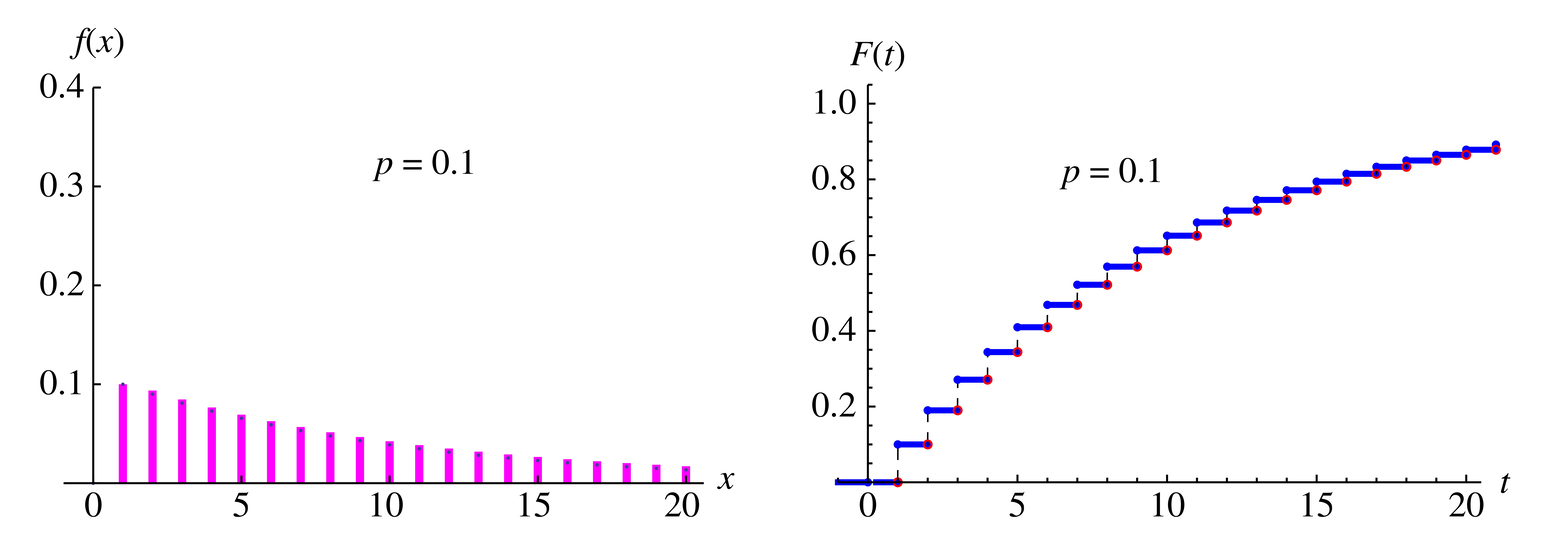
\includegraphics[width=1\linewidth]{geom.png}\caption{Geométrica $G(p)$}
		Número $n$ de ensayos de Bernoulli independientes con la misma probabilidad de éxito $p$, hasta obtener el primer éxito.
		\begin{equation}
		\begin{matrix}
		f(x)=q^{x-1},\\
		x=1,2,\ldots,n;\\
		E(X)=\frac{1}{p},\ Var(X)=\frac{q}{p^2}
		\end{matrix}
		\end{equation}
	\end{subfigure}
	\begin{subfigure}[t]{.5\textwidth}
		\includegraphics[width=.95\linewidth]{negativabinominal.png}\caption{Negativa binominal $Nb(rp)$}
		Número $n$ de ensayos de Bernoulli independientes con la misma probabilidad de éxito $p$, hasta obtener resultado número $r$.
		\begin{equation}
		\begin{matrix}
		f(x)=\binom{x-1}{r-1}p^rq^{x-r},\\
		r=r,r+1,r+2,\ldots,n;\\
		E(X)=\frac{r}{p},\ Var(X)=\frac{rq}{p^2}
		\end{matrix}
		\end{equation}
	\end{subfigure}\ \ \ \ 
\begin{subfigure}[t]{.5\textwidth}
		\includegraphics[width=.95\linewidth]{hyperg.png}\caption{Hipergeométrica $h(n;a,b)$}
		Muestra aleatoria tamaño $n$ de ``bolas blancas'' no reemplazada de un contenedor con $a$ blancas y $b$ negras.
		\begin{equation}
		\begin{matrix}
		f(x)=P(X=x)=\frac{num}{den}\\
		y\\
		z
		\end{matrix}
		\end{equation}
	\end{subfigure}	
	\begin{subfigure}[t]{.5\textwidth}
		\includegraphics[width=.95\linewidth]{gama.png}
		\caption{$\Gamma$}
	\end{subfigure}\ \ \ \ 
\begin{subfigure}[t]{.5\textwidth}\centering
		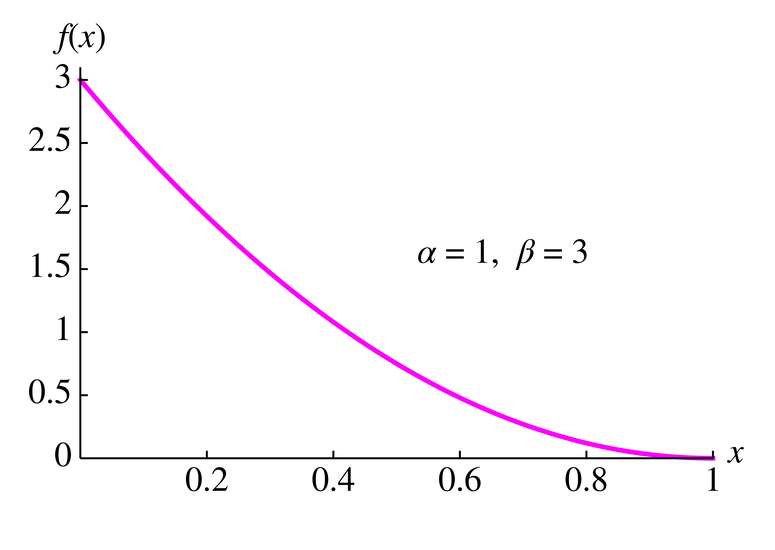
\includegraphics[width=.95\linewidth]{beta.png}\caption{Beta}
		blablabla
		\begin{equation}
		\begin{matrix}
		x\\
		y\\
		z
		\end{matrix}
		\end{equation}
	\end{subfigure}	
	\begin{subfigure}[t]{.5\textwidth}
		\includegraphics[width=.95\linewidth]{epsilon_lambda.png}
		\caption{$\epsilon(\lambda)$}
	\end{subfigure}\ \ \ \ 
\begin{subfigure}[t]{.5\textwidth}
		\includegraphics[width=.95\linewidth]{normal.png}\caption{Normal}
		blablabla
		\begin{equation}
		\begin{matrix}
		x\\
		y\\
		z
		\end{matrix}
		\end{equation}
	\end{subfigure}	
	\begin{subfigure}[t]{.5\textwidth}
		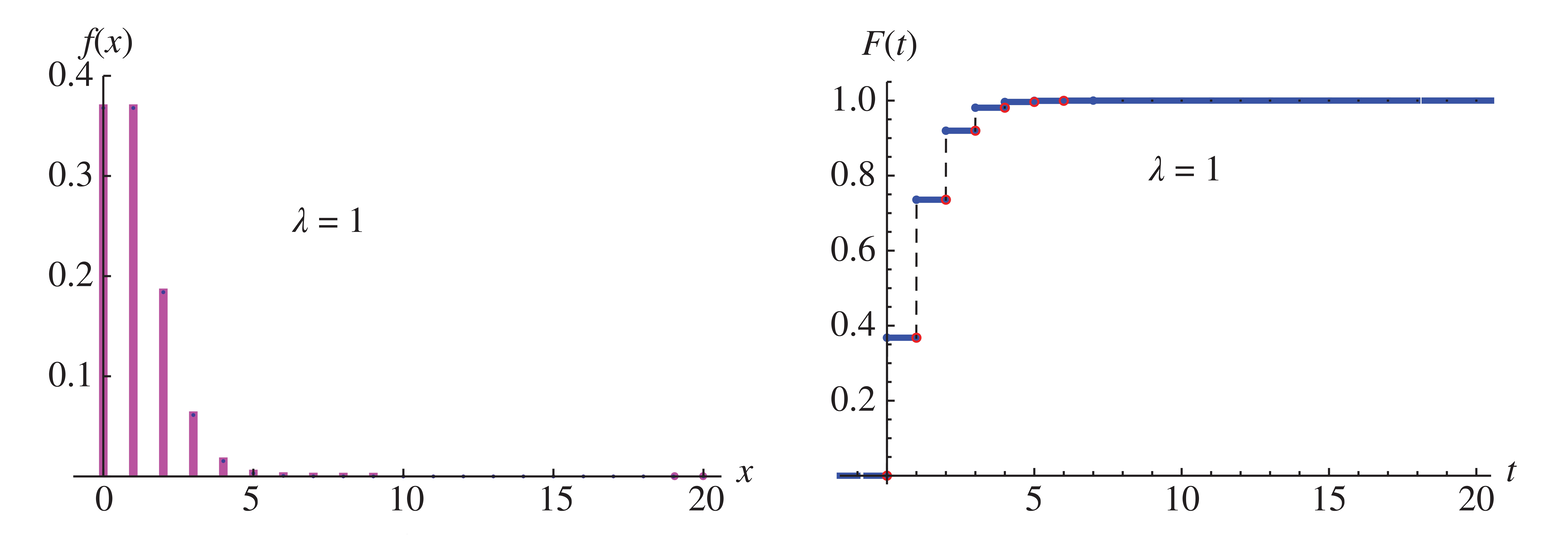
\includegraphics[width=.95\linewidth]{poisson.png}\caption{Poisson}
		blablabla
		\begin{equation}
		\begin{matrix}
		x\\
		y\\
		z
		\end{matrix}
		\end{equation}
	\end{subfigure}\ \ \ \ 
\begin{subfigure}[t]{.5\textwidth}
		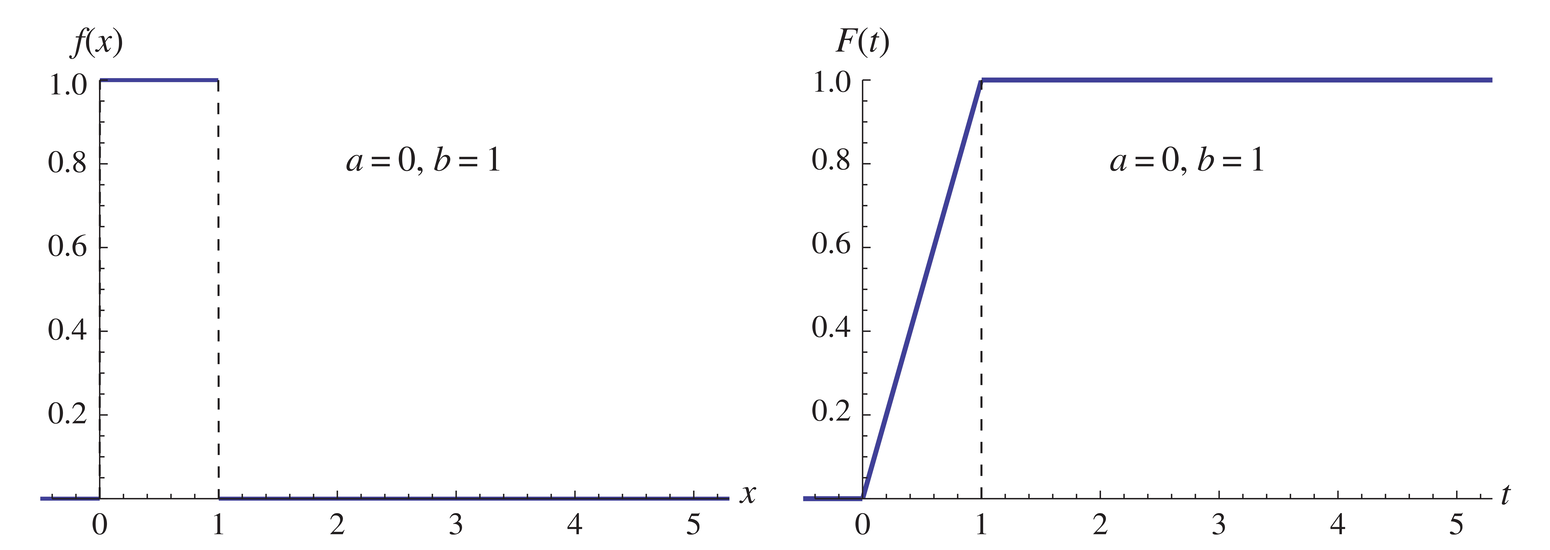
\includegraphics[width=.95\linewidth]{uniforme.png}\caption{Uniforme}
		blablabla
		\begin{equation}
		\begin{matrix}
		x\\
		y\\
		z
		\end{matrix}
		\end{equation}
	\end{subfigure}
\end{figure}
\#\#\#\#\#\#\#\#\#\#\#\#\#\#\#\#\#\#\#\#\#\#\#\#\#\#\#\#\#\#\#\#\#\#\#\#\#\#\#\#
\begin{center}sup\end{center}

\#\#\#\#\#\#\#\#\#\#\#\#\#\#\#\#\#\#\#\#\#\#\#\#\#\#\#\#\#\#\#\#\#\#\#\#\#\#\#\#\\
\section {Objetivos}
\subsection {General}
Haciendo uso de las ciencias de la computación, las herramientas matemáticas de estadística y métodos de aprendizaje autónomo, se busca obtener información cuantitativa de textos. La fuente de información será redes sociales, cadenas noticiosas y audio de programas de capacitación, para inferir posiciones, tendencias, comportamientos o razones de grupos sociales. El de trabajo es clasificación, estimación, detección y comprobación.
\subsection {Particulares}
\begin{enumerate}
    \item Desarrollar un modelo de base de datos que permita la captura de categorías para un determinado problema, los elementos de identificación de cada categoría, el origen de la información y su correlación.
    \item Construir una estructura de datos que capte la estimación o valores esperados para el procesamiento de textos.
    \item Elaborar un sistema de objetos para el soporte de los elementos de aprendizaje autónomo.
    \item Generar los elementos de captura de textos para su almacenamiento y procesamiento.
    \item Elaborar un modelo estadístico que permita comprobar las estimaciones a partir de los datos y en consecuencia realizar un ajuste en los parámetros usados para el aprendizaje autónomo.
    \item Producir los reportes con un análisis estadístico que faciliten la interpretación de resultados y den pauta para la obtención del conocimiento de interés.
\end{enumerate}
\section {Metas científicas}
La meta de este proyecto es -la integración -de elementos de estad, ciencia comp, apr autónomo(ML) para procesamiento de lenguage natural (PLN).
\section {Metodología científica}
\section {Grupo de trabajo}
\section {Grupo de trabajo}
\begin{itemize}
	\item Dr. José Emilio Quiroz Ibarra, Director.\\
Universidad Iberoamericana.
	\item Dra. Alma Rocío Sagaceta Mejía, Co-directora.\\
Universidad Autónoma Metropolitana.
	%\item Mtra. Paloma Alejandra Vilchis León\\
	%Universidad Tecnológica de México*\notad{preguntar}, Tutoría.
\end{itemize}
\section {Infraestructura disponible para el proyecto}
Laboratorios y equipos disponibles en la Universidad Iberoamericana Ciudad de México.

Desktop
CPU Intel i7 (ó AMD Ryzen 7)
RAM 32 GB
Almacenamiento 2TB SSD (ó 256 SSD y 2TB HDD)

Servidor
Renta de servicio virtual en Google Cloud, Amazon AWS o Microsoft Azure, entre otros. (adquirir uno, al menos $50k).
\section {Cronograma de actividades}
cronograma
\section {Resultados comprometidos}
Publicación
\section {Visto bueno}
Vo.Bo.
\section {Referencias}
\printbibliography[heading=none]
\end{document}